\documentclass{beamer}

\mode<presentation> {
  \usetheme{Dresden}
  \usecolortheme{beaver}
  \setbeamercovered{transparent}
  \setbeamercolor*{item}{fg=darkred}
  \setbeamercolor*{block title}{fg=darkred}
}

\usepackage{ucs}
\usepackage[utf8x]{inputenc}
\usepackage[czech]{babel}
\usepackage{palatino}
\usepackage{graphicx}

\title{40~GbE směrovač pro operační systém GNU/Linux}
\author{Bc. Josef Luštický}
\date{1.~6.~2015}

\begin{document}

\begin{frame}
  \titlepage
\end{frame}

% Numbering
\expandafter\def\expandafter\insertshorttitle\expandafter{%
  \insertshorttitle\hfill%
  \insertframenumber\,/\,\inserttotalframenumber}

% Do not count the Titlepage in frame numbers
\addtocounter{framenumber}{-1}

\begin{frame}{Obsah}
	\begin{itemize}
		\item 40~GbE - IEEE 802.3ba
		\item Zpracování paketů L2-L3 v Linuxu
		\item Analýza
		\item Setup - zapojení, konfigurace
		\item Měření - výsledky
		\item Závěr
	\end{itemize}
\end{frame}

\begin{frame}{Růst výkonu}
	\begin{figure}
			\centering
			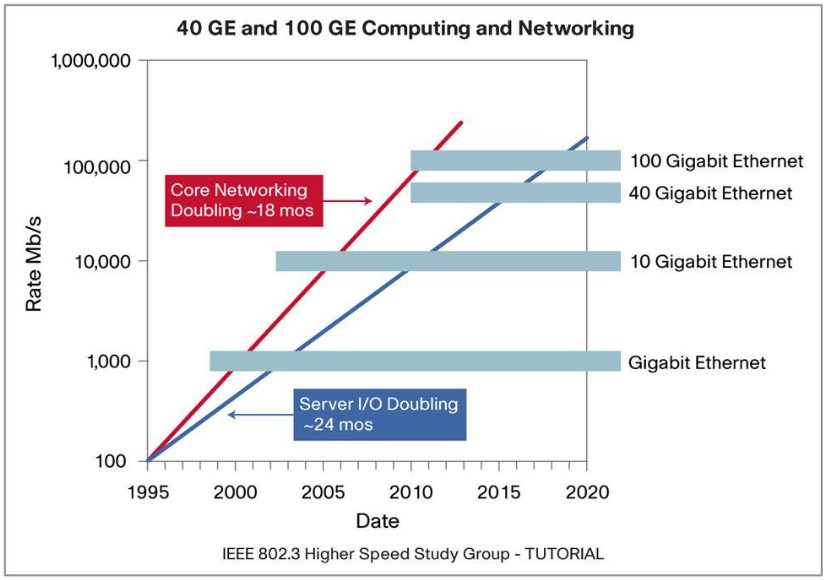
\includegraphics[width=8cm,keepaspectratio]{fig/performance-gap.png}
		\end{figure}
\end{frame}

\begin{frame}{40~GbE}
	\begin{itemize}
		\item Propustnost - 4.6~GB/s (PCIe 3.0 x8 zvládne 7.9~GB/s)
		\item Frame rates - 3.26 - 59.5~Mpps (MTU 1518 / 64~B) \\
		307.6 / 16.8~ns (51 cyklů na 3~GHz CPU)
		\item Kompatibilita - RHEL 7, 6.6, plánovaný 40GBASE-T s dosahem 30m
	\end{itemize}
\end{frame}

\begin{frame}{Síťový stack v Linuxu}
	\begin{figure}
			\centering
			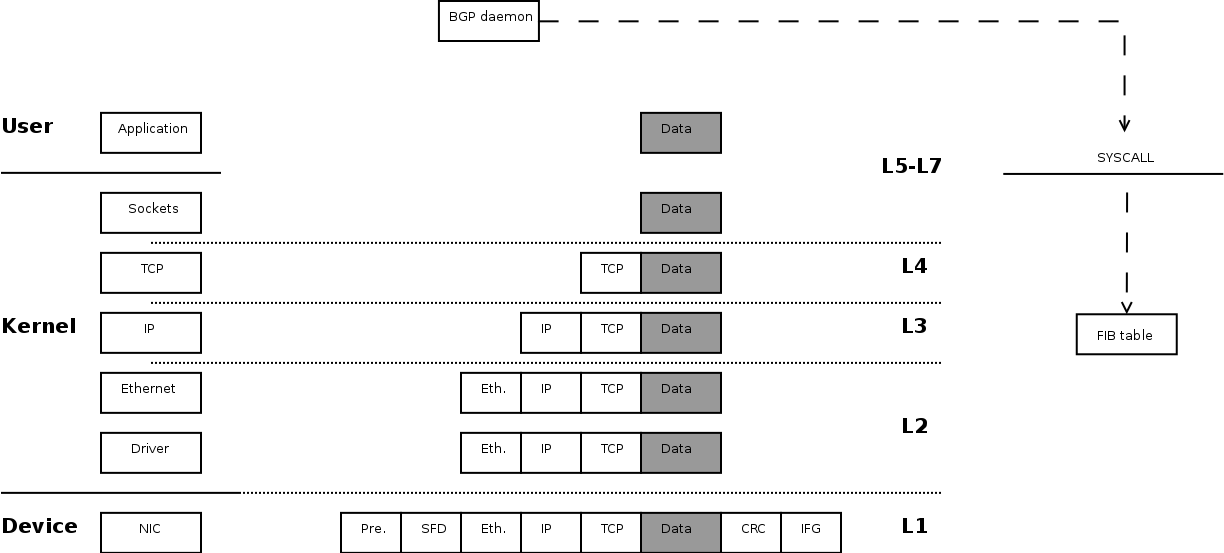
\includegraphics[width=8cm,keepaspectratio]{fig/layers.png}
		\end{figure}
\end{frame}




\begin{frame}{Velikost rámců v AMS-IX}
	\begin{figure}
			\centering
			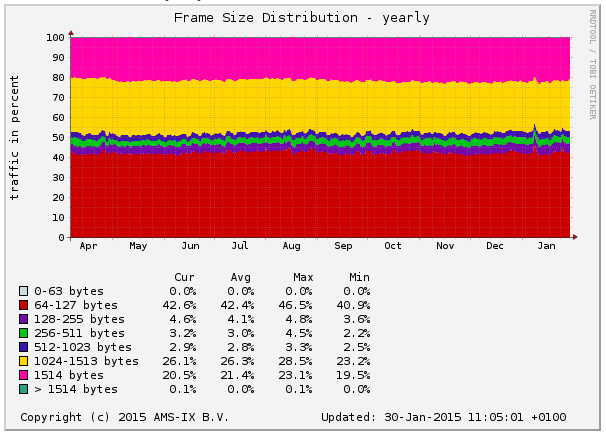
\includegraphics[width=8cm,keepaspectratio]{fig/amsix.png}
		\end{figure}
\end{frame}

\end{document}
